\section{Results}
\label{chapter:03}

% block-id: 03.analytic.heading
\hypertarget{03.analytic.heading}{}
\subsection{Round-wire internal-field calibration}

% block-id: 03.analytic.p1
\hypertarget{03.analytic.p1}{}
The radial current and internal impedance of a long straight round wire follow \eqref{eq:E03}. At 200 kHz, the skin depth δ=\metric{skin_depth} mm is approximately 0.148 times the radius, and current concentrates near the surface. DC resistance is \metric{q1_rdc} mΩ/m, AC resistance is \metric{q1_rac} mΩ/m, and Rac/Rdc=3.64720, giving a loss of \metric{q1_loss} W/m. The radial profiles and cross-sectional magnitude appear in Fig.~\ref{fig:q1_profile} and Fig.~\ref{fig:q1_cross_section}. Radial phase is continuously unwrapped, showing the amplitude attenuation and phase change associated with skin diffusion. The analytical impedance concerns the conductor's internal field.

% block-id: 03.equation.E03
\hypertarget{03.equation.E03}{}
\hypertarget{E03}{}
\begin{equation}
\begin{gathered}
\delta=(\pi f\mu\sigma)^{-1/2} \\
\kappa=(1+j)/\delta \\
J_z(r)=\frac{I_t\kappa I_0(\kappa r)}{2\pi a I_1(\kappa a)} \\
z_{\mathrm{int}}=\frac{\kappa I_0(\kappa a)}{2\pi a\sigma I_1(\kappa a)}
\end{gathered}
\tag{6}\label{eq:E03}
\end{equation}

% block-id: 03.figure.q1_profile
\hypertarget{03.figure.q1_profile}{}
\begin{figure*}[!htbp]
\centering
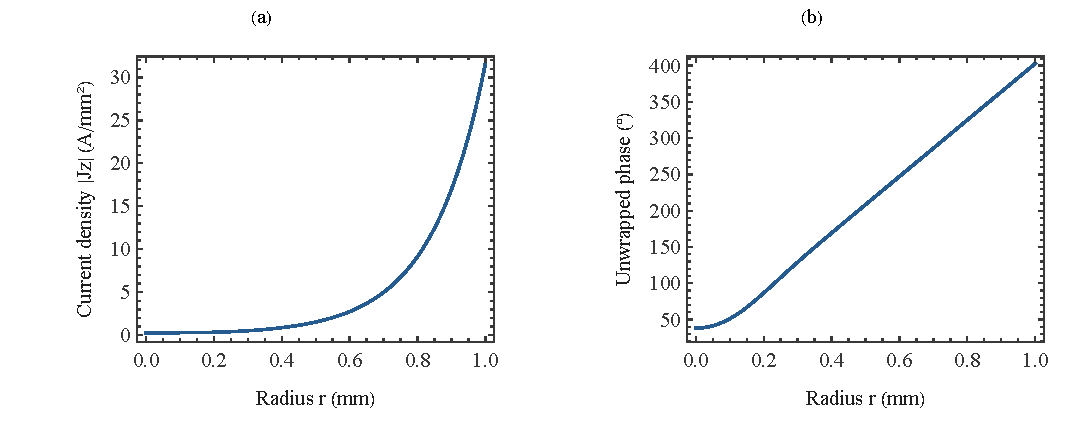
\includegraphics[width=\linewidth,height=.72\textheight,keepaspectratio]{../../assets/en/q1_profile.pdf}
\caption{Round-wire radial current magnitude and phase. The copper conductor has diameter 2 mm and carries 20 A RMS at 200 kHz. (a) RMS magnitude; (b) continuously displayed phase.}
\label{fig:q1_profile}
\end{figure*}

% block-id: 03.analytic.p2
\hypertarget{03.analytic.p2}{}
Independent two-dimensional disk diffusion uses three meshes with 353, 1389, and 5573 nodes, normalized by total complex current. With refinement, relative Rac error against analysis decreases from 7.05×10⁻³ to 2.30×10⁻⁴ and finally 1.79×10⁻⁶. The finest-grid relative power-integral difference is 3.07×10⁻⁶, as shown in Fig.~\ref{fig:q1_fem_error}. These results verify discretization, normalization, and power postprocessing for the isolated round-wire internal-field problem. The cross-sectional illustration uses linear interpolation of analytical radial samples and an axisymmetric mapping; subsequent multistrand models use their actual conductor field solutions.

% block-id: 03.figure.q1_cross_section
\hypertarget{03.figure.q1_cross_section}{}
\begin{figure}[!htbp]
\centering
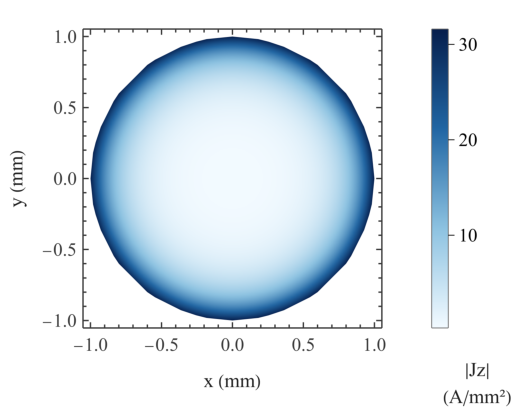
\includegraphics[width=\linewidth,height=.72\textheight,keepaspectratio]{../../assets/en/q1_cross_section.pdf}
\caption{Analytical round-wire cross-sectional magnitude. The copper conductor has diameter 2 mm and carries 20 A RMS at 200 kHz. The color scale represents axial RMS current density.}
\label{fig:q1_cross_section}
\end{figure}

% block-id: 03.figure.q1_fem_error
\hypertarget{03.figure.q1_fem_error}{}
\begin{figure}[!htbp]
\centering
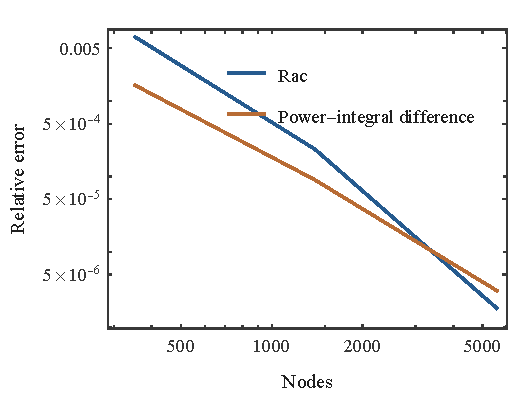
\includegraphics[width=\linewidth,height=.72\textheight,keepaspectratio]{../../assets/en/q1_fem_error.pdf}
\caption{Round-wire two-dimensional calibration errors. The copper conductor has diameter 2 mm and carries 20 A RMS at 200 kHz. Three grids and independent power integrals concern the same internal-field problem.}
\label{fig:q1_fem_error}
\end{figure}

% block-id: 03.coax_results.heading
\hypertarget{03.coax_results.heading}{}
\subsection{Common-terminal currents and loss in a 640-strand straight bundle}

% block-id: 03.quantitative.p1
\hypertarget{03.quantitative.p1}{}
The actual copper cross-section of the two-dimensional 640-strand model is \metric{coax_area} mm². Bundle AC resistance is \metric{coax_rac} mΩ per axial metre, bundle loss is \metric{coax_bundle_loss} W per axial metre, and return loss is \metric{coax_return_loss} W per axial metre. Separate integration identifies dissipation in the bundle and return. The common axial terminal field is \metric{coax_voltage_re}+j(\metric{coax_voltage_im}) V/m. Complex strand currents sum to 20 A RMS, while their normalized RMS complex-current deviation is \metric{coax_spread}, demonstrating substantial interstrand differences in this common-terminal straight bundle.

% block-id: 03.coax_results.p2
\hypertarget{03.coax_results.p2}{}
Fig.~\ref{fig:coax640_currents} shows current magnitude and phase by physical strand identity, with It/N as the equal-current reference. Magnitude and phase jointly determine each strand's contribution to total transport current, so current sharing is evaluated using complex currents. Fig.~\ref{fig:coax640_fields} gives the corresponding cross-sectional fields, connecting strand statistics with spatial position. In this axially invariant straight bundle, the skin-effect scale within each fine strand coexists with collective current redistribution caused by magnetic coupling across the bundle. Longitudinal transposition requires a separate representation of position changes.

% block-id: 03.figure.coax640_currents
\hypertarget{03.figure.coax640_currents}{}
\begin{figure*}[!htbp]
\centering
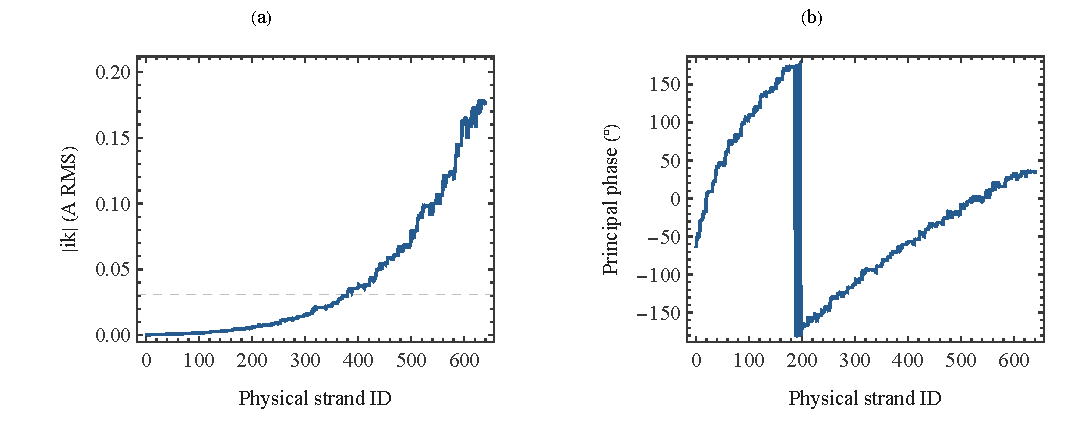
\includegraphics[width=\linewidth,height=.72\textheight,keepaspectratio]{../../assets/en/coax640_currents.pdf}
\caption{640-strand common-terminal complex current sharing. (a) Magnitude; (b) phase, ordered by physical strand identity.}
\label{fig:coax640_currents}
\end{figure*}

% block-id: 03.figure.coax640_fields
\hypertarget{03.figure.coax640_fields}{}
\begin{figure*}[!htbp]
\centering
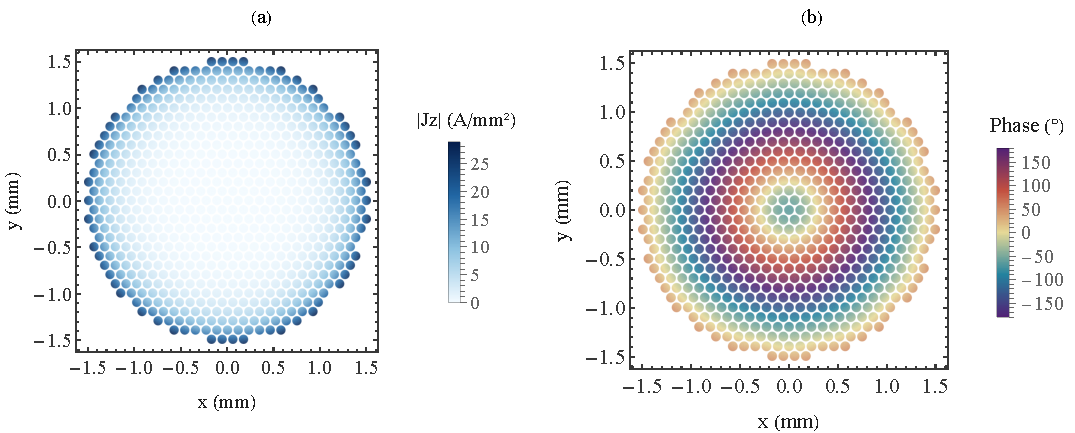
\includegraphics[width=\linewidth,height=.72\textheight,keepaspectratio]{../../assets/en/coax640_fields.pdf}
\caption{640-strand two-dimensional cross-sectional current density. (a) RMS magnitude; (b) phase, with material markers identifying strands.}
\label{fig:coax640_fields}
\end{figure*}

% block-id: 03.coax_results.p1
\hypertarget{03.coax_results.p1}{}
Three meshes and variations of return distance and exterior domain complete 23 checks. The final mesh refinement changes Rac by 0.011902\%; return-distance and exterior-domain changes are 0.000495\% and 0.000270\%, respectively, as shown in Fig.~\ref{fig:coax640_mesh}. These changes remain below the 1\% comparison target over the tested perturbations, supporting numerical stability of the specified two-dimensional common-terminal result. Its applicability is a straight two-dimensional bundle with a controlled return; finite end regions and longitudinal coupling in actual wound structures require further verification.

% block-id: 03.figure.coax640_mesh
\hypertarget{03.figure.coax640_mesh}{}
\begin{figure}[!htbp]
\centering
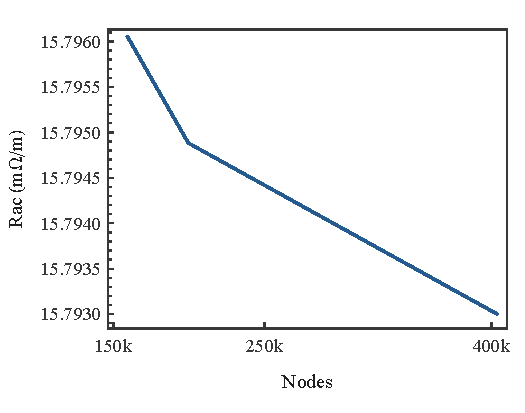
\includegraphics[width=\linewidth,height=.72\textheight,keepaspectratio]{../../assets/en/coax640_mesh.pdf}
\caption{640-strand mesh and boundary sensitivities. Mesh, return, and exterior tests each vary one factor.}
\label{fig:coax640_mesh}
\end{figure}

% block-id: 03.peec_results.heading
\hypertarget{03.peec_results.heading}{}
\subsection{Length and integration sensitivity of longitudinal PEEC}

% block-id: 03.peec_results.p1
\hypertarget{03.peec_results.p1}{}
For the 1264-degree-of-freedom model, resistances at 0.16, 0.32, and 0.64 m are 19.8992, 19.9586, and 19.9885 mΩ per axial metre. Consecutive length changes are 0.298640\% and 0.149482\%. The 5024-degree-of-freedom model changes by 0.148730\% from 0.32 to 0.64 m, as shown in Fig.~\ref{fig:peec_length}. Resistance changes decrease with increasing length, and all tested increments are below 1\%. The sequence characterizes sensitivity over the 0.16–0.64 m interval.

% block-id: 03.peec_results.p2
\hypertarget{03.peec_results.p2}{}
At 5024 degrees of freedom, Lz=0.64 m, mutual order q=4, and self-integration settings 12/10, Rac=\metric{peec_rac} mΩ per axial metre, Rac/Rdc=3.64472, and loss is 8.00510 W per axial metre. Resistance differs by 0.044582\% from the equal-area Bessel reference for this discretization. Fig.~\ref{fig:peec_cross_section} reconstructs the cross-sectional current distribution from saved filament currents and square cells, showing surface concentration within the conductor. These degrees of freedom discretize a continuous conductor; their current variation has a different meaning from current sharing among insulated strands.

% block-id: 03.figure.peec_length
\hypertarget{03.figure.peec_length}{}
\begin{figure}[!htbp]
\centering
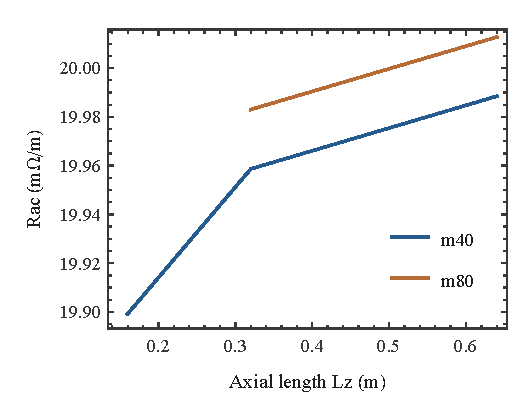
\includegraphics[width=\linewidth,height=.72\textheight,keepaspectratio]{../../assets/en/peec_length.pdf}
\caption{Longitudinal PEEC length sensitivity. Resistance per axial length is compared at archived lengths for the same cross-section.}
\label{fig:peec_length}
\end{figure}

% block-id: 03.figure.peec_cross_section
\hypertarget{03.figure.peec_cross_section}{}
\begin{figure}[!htbp]
\centering
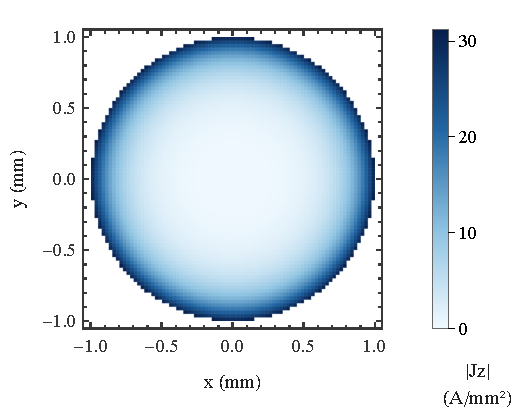
\includegraphics[width=\linewidth,height=.72\textheight,keepaspectratio]{../../assets/en/peec_cross_section.pdf}
\caption{Longitudinal PEEC cross-sectional current. Complex currents in square volume filaments reconstruct the RMS magnitude.}
\label{fig:peec_cross_section}
\end{figure}

% block-id: 03.peec_results.p3
\hypertarget{03.peec_results.p3}{}
Results for mutual order q=4\(\to\)6\(\to\)8 and self settings 10/8\(\to\)12/10 appear in Fig.~\ref{fig:peec_sensitivity}. Across both model sizes, the largest relative resistance change from mutual integration is 1.21×10⁻⁵ and the largest relative complex-current change is 1.60×10⁻⁵. Corresponding maxima for self integration are 6.75×10⁻¹¹ and 7.10×10⁻¹¹. Coarse-to-fine cross-sectional resistance changes at 0.32 and 0.64 m are 0.122127\% and 0.121376\%, respectively, and include changes in actual area. Thus integration settings have a smaller effect than length and cross-sectional discretization in these tests. Analytical references and sensitivities jointly support resistance calculation within the longitudinal model; actual end regions and transverse-current errors remain model-level research questions.

% block-id: 03.figure.peec_sensitivity
\hypertarget{03.figure.peec_sensitivity}{}
\begin{figure}[!htbp]
\centering
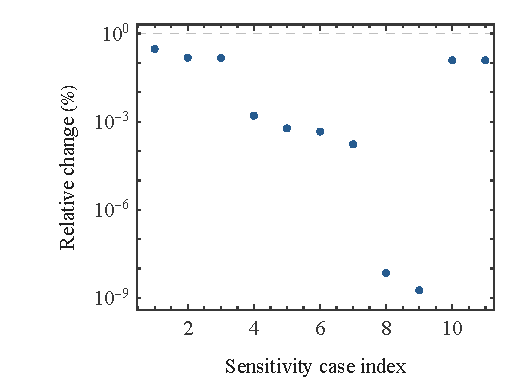
\includegraphics[width=\linewidth,height=.72\textheight,keepaspectratio]{../../assets/en/peec_sensitivity.pdf}
\caption{Longitudinal PEEC integration sensitivity. Mutual order and self accuracy are compared in separate single-factor tests.}
\label{fig:peec_sensitivity}
\end{figure}

% block-id: 03.compute.heading
\hypertarget{03.compute.heading}{}
\subsection{CPU/GPU numerical comparison and computational scale}

% block-id: 03.compute.p1
\hypertarget{03.compute.p1}{}
With identical model, discretization, and integration settings, the 5024-degree-of-freedom CPU/GPU partial-inductance matrices differ relatively by 7.48×10⁻¹⁶ and their complex currents by 7.78×10⁻¹⁴. The 1264-degree-of-freedom case also meets the 10⁻¹⁰ comparison threshold, as shown in Fig.~\ref{fig:gpu_equivalence}. These results establish numerical agreement between the two implemented algorithms for the compared matrices and port solutions. Performance comparisons additionally require matching timing boundaries; stage times and resource samples are retained, while physical conclusions rely on the model checks described above.

% block-id: 03.compute.p2
\hypertarget{03.compute.p2}{}
Fig.~\ref{fig:resource_memory} shows sampled memory usage for identifiable owned process trees; short peaks between samples may exceed the displayed curve. At larger scales, the 9856-degree-of-freedom case retains recoverable partial currents and related results, while its complete matrix, common voltage and full-field coverage are itemized in the data inventory. Cases with 20108 or more degrees of freedom record resource requirements and termination boundaries. These records inform the cost of further computation; complete numerical verification rests on cases with the corresponding acceptance data.

% block-id: 03.figure.gpu_equivalence
\hypertarget{03.figure.gpu_equivalence}{}
\begin{figure}[!htbp]
\centering
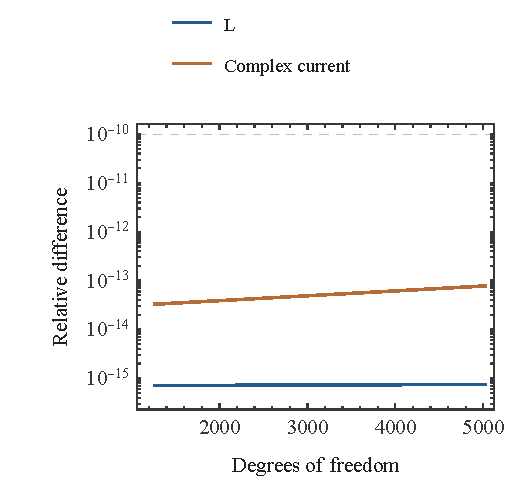
\includegraphics[width=\linewidth,height=.72\textheight,keepaspectratio]{../../assets/en/gpu_equivalence.pdf}
\caption{CPU/GPU same-model numerical comparison. Relative matrix and complex-current differences use identical discretization and integration.}
\label{fig:gpu_equivalence}
\end{figure}

% block-id: 03.figure.resource_memory
\hypertarget{03.figure.resource_memory}{}
\begin{figure}[!htbp]
\centering
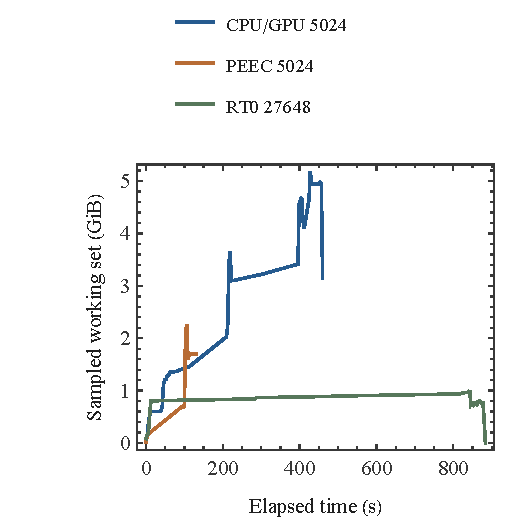
\includegraphics[width=\linewidth,height=.72\textheight,keepaspectratio]{../../assets/en/resource_memory.pdf}
\caption{Attributable process-tree resource curves. Curves use archived time and memory samples.}
\label{fig:resource_memory}
\end{figure}
